\documentclass{article}

\usepackage[T1]{fontenc} % Umożliwia korzystanie z fontów o kodowaniu T1, które obsługują znaki specjalne używane w językach europejskich.
\usepackage[polish]{babel} % Dostosowuje formatowanie dokumentu do zasad języka polskiego (np. łamanie wierszy, tytuły sekcji).
\usepackage[utf8]{inputenc} % Umożliwia korzystanie z kodowania UTF-8, które obsługuje znaki specjalne i diakrytyczne.
\usepackage{graphicx} % Umożliwia wstawianie obrazów do dokumentu.
\usepackage{subcaption} % Umożliwia tworzenie podpisów dla podobrazów.
\usepackage[margin=2cm]{geometry} % Umożliwia dostosowanie marginesów dokumentu.
\usepackage{listings} % Umożliwia wstawianie kodu źródłowego do dokumentu z odpowiednim formatowaniem.
\usepackage{color} % Umożliwia korzystanie z kolorów w dokumencie.
\usepackage{amsmath} % Rozszerza możliwości formatowania równań matematycznych.
\usepackage{tcolorbox} % Umożliwia tworzenie kolorowych ram dookoła tekstu.
\usepackage{systeme} % Umożliwia tworzenie systemów równań.
\usepackage{indentfirst} % Powoduje, że pierwszy akapit po tytule sekcji jest wcięty.
\usepackage{dsfont} % Umożliwia korzystanie z dodatkowych fontów, np. dla oznaczeń zbiorów liczbowych.
\usepackage{etoolbox} % Pozwala modyfikować pakiety UŻYWAĆ OSTROŻNIE
\usepackage{blindtext} % Pozwala automatycznie pisać blok lorem ipsum
\usepackage{fancyhdr} % Pozwala na stopki u góry i na dole strony
\usepackage{hyperref} % Umożliwia używanie hyperlinków
\usepackage[justification=centering]{caption}
\hypersetup{
  colorlinks = true,
  linkcolor = black,
  urlcolor = blue,
  pdftitle = {Sprawozdanie z Laboratorium 3} 
}
\patchcmd{\section}{\thispagestyle{plain}}{\thispagestyle{fancy}}{}{}

\definecolor{red}{RGB}{245, 63, 60}
\definecolor{blue}{RGB}{59, 69, 245}
\definecolor{green}{RGB}{59, 245, 117}
\definecolor{yellow}{RGB}{245, 207, 59}

\begin{document}
  \pagestyle{fancy} % pozwala korzystać z pakietu fancyhdr
  \fancyhf{} % clear existing header/footer entries
  \fancyfoot[C]{\thepage}
  \renewcommand{\headrulewidth}{0pt} % Usuń linię na górze strony
  \renewcommand{\footrulewidth}{0.4pt} % Dodaj linię na dole strony  
  \addtolength{\footskip}{0cm} % Zmienia pozycję linii w stopce

  \title{Elektronika Cyfrowa \\ {\large Sprawozdanie z Laboratorium 3}}
  \date{10.04.2024}
  \author{Tomasz Dziób\\{\small Grupa 15}}
  \maketitle

  % Ustawienie Spisu treści do paragrafów 
  \setcounter{tocdepth}{4} % Uwzględnij do typu \paragraph in Spisie treści
  \setcounter{secnumdepth}{4} % Numerowanie do typu \paragraph
  \tableofcontents
  \pagebreak
  \section{Wstęp teoretyczny}
  Poniższe sprawozdanie dotyczy dotyczy trzecich zajęć których głównym celem było zapoznanie się z działaniem wzmacniaczów operacyjnych oraz przerzutników. 
    \subsection{Sprzężenie zwrotne}
      \textit{Sprzężenie zwrotne} --- reakcja, będąca bezpośrednim oddziaływaniem sygnałów stanu końcowego na sygnały wejściowe. Część sygnału wyjściowego zwana sygnałem zwrotnym, zostaje skierowana do wejścia układu i zsumowana  z sygnałem wejściowym.

      Głównym elementem elektronicznym, w którym stosuje się sprzężenie zwrotne jest wzmacniacz sygnału.

      \begin{figure}[!ht]
        \begin{minipage}{.5\textwidth}
            \centering
            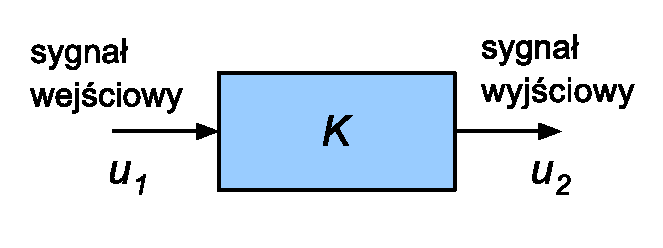
\includegraphics[scale=0.75]{grafiki/bez_sprzezenia.eps}
            \caption{Schemat wzmacniacza \textcolor{red}{\underline{bez}} sprzężenia zwrotnego,
            \\Źródło: \href{https://spe.if.uj.edu.pl/literatura}{Strona wykładów}}
        \end{minipage}
        \begin{minipage}{.5\textwidth}
            \centering
            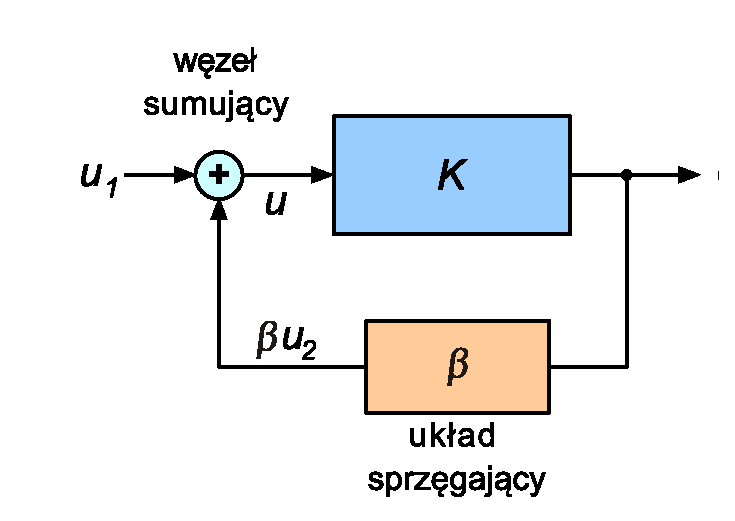
\includegraphics[scale=0.75]{grafiki/z_sprzezeniem.eps} 
            \caption{Schemat wzmacniacza ze sprzężeniem zwrotnym,
            \\Źródło: \href{https://spe.if.uj.edu.pl/literatura}{Strona wykładów}}
        \end{minipage}
      \end{figure}

      Wzór na wzmocnienie układu bez sprzężenia zwrotnego:
      \begin{equation}
        u_2(t) = K u_1(t)
      \end{equation}
      Natomiast podczas użycia sprzężenia zwrotnego prezentuje się on nastepująco:
      \begin{equation}
        u_2(t) = \frac{Ku_1}{1 - \beta K }
      \end{equation}



      Sprzężenie zwrotne możemy podzielić dwa rodzaje:
      \begin{itemize}
        \item Ujemne sprzężenie zwrotne --- Sytuacja gdy fazy sygnału wejściowego i sygnału sprzężenia zwrotnego są przeciwne. Charakteryzuje się dużą stabilnością pracy układu. Zazwyczaj używane w wzmacniaczach.
        
        \item Dodatnie sprzężenie zwrotne --- Sytuacja gdy fazy sygnału wejściowego i sygnału sprzężenia zwrotnego są zgodne. W układach takich dzięki silnemu sprzężeniu następuje generacja drgań co wykorzystywane jest do budowy generatorów(przerzutnikach).
      \end{itemize}

    \subsection{Wzmacniacz operacyjny}
      Wzmacniacz o bardzo dużym wzmocnieniu napięciowym, który posiada dwa wejścia i jedno wyjście. Wyróżniamy dwa wejścia:
      \begin{enumerate}
        \item[\textcolor{red}{\textbf{(-)}}] \textcolor{red}{\textbf{Wejście odwracające}} --- Przesuwa ono sygnał wyjściowy w fazie o $180^\circ$ względem sygnału przyłożonego do tego wejścia
        \item[\textcolor{green}{\textbf{(+)}}] \textcolor{green}{\textbf{Wejście nieodwracające}} --- Sygnał wyjściowy jest zgodny w fazie z sygnałem podanym na to wejście
      \end{enumerate}

      \begin{figure}[!ht]
        \centering
        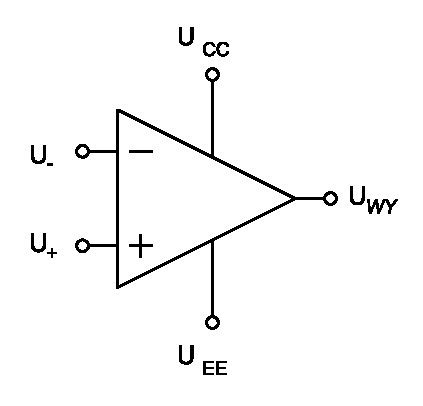
\includegraphics[scale=0.70]{grafiki/wmacniacz_symbol.eps}
        \caption{Powszechnie stosowany symbol graficzny do oznaczania wzmacniacza operacyjnego,
        \\Źródło: \href{https://pl.wikipedia.org/wiki/Wzmacniacz_operacyjny}{Wikipedia}}
      \end{figure}
      \pagebreak
      Wejścia $U_{CC}$ oraz $U_{EE}$ to wejścia napięcia zasilania wzmacniacza.
      
      Wzór na napięcie wyjściowe:
      \begin{equation}
        U_{WY} = K(U_+ - U_-)
      \end{equation}

      \subsubsection{Wzmacniacz odwracający fazę}

      Wzmacniacz odwracający fazę to specyficzny typ wzmacniacza operacyjnego, który na wyjściu daje napięcie o odwrotnym znaku (czyli o przeciwnej fazie) w stosunku do napięcia wejściowego.

      \begin{figure}[!ht]
        \centering
        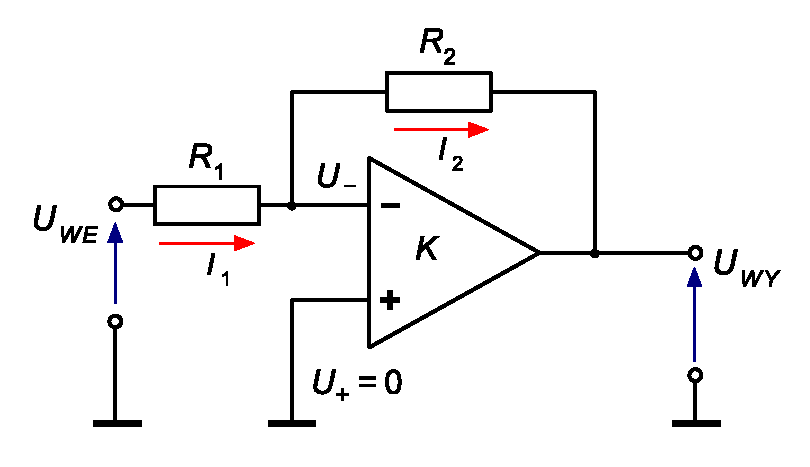
\includegraphics[scale=0.70]{grafiki/odwracajacy_faze.eps}
        \caption{Schemat prezentujący budowę wzmacniacza odwracającego fazę,
        \\Źródło: \href{https://spe.if.uj.edu.pl/literatura}{Strona wykładów}}
        \label{fig1:schemat_odwracajacego}
      \end{figure}

      Wzmacniacz ten składa się ze wzmacniacza operacyjnego oraz dwóch oporników: opornika wejściowego i opornika sprzężenia zwrotnego.
      Napięcie wyjściowe zależy bezpośrednio od różnicy rezystacji $R_1$ oraz $R_2$:
      \begin{equation}
        U_{WY} = - \frac{R_2}{R_1}U_{WE}
        \label{eq1:odwracajacy}
      \end{equation}

      \subsubsection{Wzmacniacz sumujący}
        Kolejną alternacją wzmacniacza odwracająego fazę jest wzmacniacz sumujący. Wykonuje on operację sumowania (dodawania) kolejnych sygnałów wejściowych.

        \begin{figure}[!ht]
          \centering
          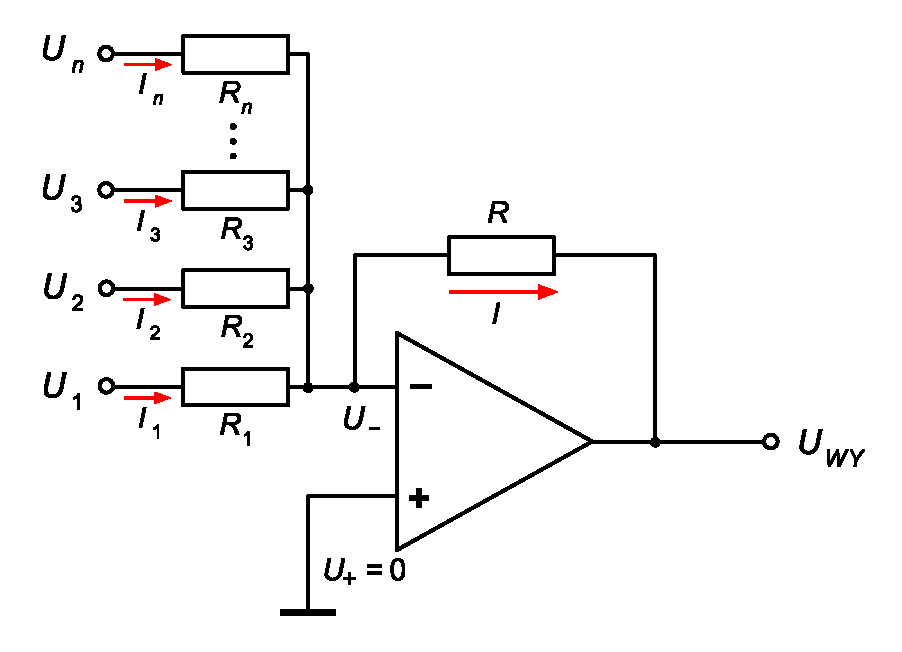
\includegraphics[scale=0.70]{grafiki/sumujacy.eps}
          \caption{Schemat prezentujący budowę sumatora napięć,
          \\Źródło: \href{https://spe.if.uj.edu.pl/literatura}{Strona wykładów}}
          \label{fig2:sumujacy}
        \end{figure}
        \pagebreak

        W ogólnej sytuacji napięcie wyjściowe można obliczyć:
        \begin{equation}
          U_{WY} = - R(\frac{U_1}{R_1}+\frac{U_2}{R_3}+\dots+\frac{U_n}{R_n})
          \label{eq2:sumujacy}
        \end{equation}

        Jednak gdy, 
        $R_1 = R_2 = \dots = R_n = R$, wtedy całość upraszcza się do:

        \begin{equation}
          U_{WY} = - R(U_1 + U_2 + \dots + U_n)
        \end{equation}

    \subsection{Przerzutnik}
        Są to układy elektroniczne wytwarzające wygnały prostokątne w których wysokość napięcia oznacza stan w którym znajduje się przerzutnik. Występowanie wysokiego i niskiego sygnału odpowiada przerzutnikowi dwustanowemu.

      \subsubsection{Rodzaje przerzutników}
        Rozróżniamy trzy typy przerzutników:

        \paragraph{bistabilne}
          \mbox{}\newline
          Posiadają dwa stany stabilne. Zmianę między stanami można wywołać tylko określonym sygnałem. Jest on też nazwany \textit{Przerzutnikiem Schmidta}.

          \begin{figure}[!ht]
            \begin{minipage}{.5\textwidth}
              \centering
              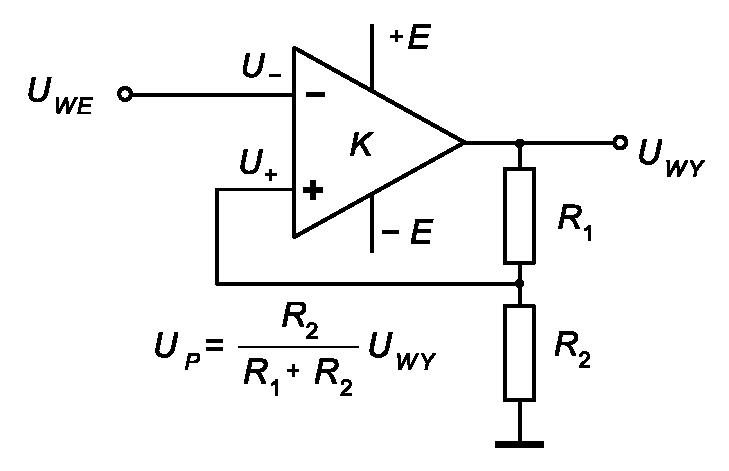
\includegraphics[scale=0.70]{grafiki/Schmidt.eps}
              \caption{Schemat prezentujący budowę przerzutnika bistabilnego,
              \\Źródło: \href{https://spe.if.uj.edu.pl/literatura}{Strona wykładów}}
              \label{fig6:Schmidt}
            \end{minipage}
            \begin{minipage}{.5\textwidth}
              \centering
              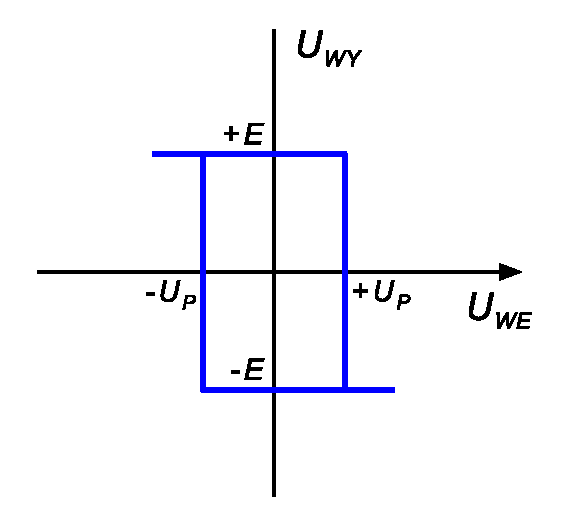
\includegraphics[scale=0.70]{grafiki/petla_histerezy.eps}
              \caption{Pętla histerezy dla układu bistabilnego,
              \\Źródło: \href{https://spe.if.uj.edu.pl/literatura}{Strona wykładów}}
              \label{fig7:histereza}
            \end{minipage}
            \end{figure}

          Napięcie wyjściowe przyjmuje wartości:
          \begin{itemize}
            \item maksymalną równą $\mathbf{+E}$
            \item minimalną równą $\mathbf{-E}$
          \end{itemize}

          Określone ona jest przez napięcie zasilania wzmacniacza, \\
          Jeżeli $\mathbf{U_- < U_+}$ to $\mathbf{W_{WY} = + E}$ \\
          Jeżeli $\mathbf{U_- > U_+}$ to $\mathbf{W_{WY} = - E}$ \\
          \pagebreak

          Pętla histerezy --- Jest to zjawisko zależności aktualnego stanu układu od stanów w poprzenich chwilach.

          Przerzutniki Schmidta wykorzystują histerezę w celu ochrony przed szumem, który w przeciwnym wypadku mógłby powodować ciągłe przełączanie między dwoma przeciwnymi stanami w sytuacji, gdy sygnał wejściowy oscyluje wokół poziomu progowego.

        \paragraph{monostabilne}
          \mbox{}\newline
          Posiadają tylko jeden stan stabilny. Przejście w stan niestabilny można uzyskać tylko ustalonym sygnałem. Przejście w drugą stronę natomiast, następuje samoczynnie bez udziału zewnętrznych sygnałów.

        \paragraph{astabilne}
          \mbox{}\newline
          Nie posiada stanów stabilnych. Układ sam wykonuje przerzuty między stanami bez udziału sygnału. Układ taki możemy nazywać generatorem przebiegów prostokątnych.

  \section{Ćwiczenia}
    \subsection{Ćwiczenie 3.1}
      Pierwsze zadanie polegało na sprawdzeniu elementów elektronicznych przez użyciem ich w zadaniach. Pomiarem który miał zostać wykonany było sprawdzenie wartości występujących na pinach zasilania wzmacniacza. \\
      Pin oznaczony "$+12V$"\mbox{} miał wartość: $\mathbf{11,88}V$, \\
      a pin "$-12V$": $\mathbf{-11,87V}$ \\
      Zgadza się to z oznaczeniami, co oznacza, że płytka funkcjonuje poprawnie.

      \begin{figure}[!ht]
        \centering
        \includegraphics[scale=0.06]{grafiki/plytka.jpg}
        \caption{Płytka zawierająca wzmacniacz,
        \\Źródło: Opracowanie własne}
      \end{figure}

      \pagebreak
    
    \subsection{Ćwiczenie 3.2}
      \subsubsection{Wzmacniacz o wzmocnieniu 10}
        Pierwszym układem który trzeba było zmontować był wzmacniacz odwracający fazę. Miał on posiadać wzmocnienie równe 10, co wiązało się z potrzebą znalezienia odpowiednich oporników, wynika to bezpośrednio ze wzoru(\ref{eq1:odwracajacy}).

        Korzystając z oznaczeń wystepujących na schemacie(\ref{fig1:schemat_odwracajacego}) użyłem oporników o wartościach, $R_1 = 10k \Omega$ a jako $R_2 = 100k \Omega$.

        Realne odczyty z oporników jakie uzyskałem prezentują się nastepująco: \\
        $R_1 \approx \mathbf{9,97k \Omega}$ \\
        $R_1 \approx \mathbf{99,6k \Omega}$ \\

        Wzmocnienie $K$ wynosi wtedy odpowiednio: \\

        \begin{equation}
          K = \frac{99,6}{9,97} \approx 9,98996
        \end{equation}

        \begin{figure}[!ht]
          \centering
          \includegraphics[scale=0.07]{grafiki/plytka_odwracajacy.jpg}
          \caption{Poprawnie zmontowany wzmacniacz odwracający fazę o wzmocnieniu 10,
          \\Źródło: Opracowanie własne}
        \end{figure}

      \subsubsection{Pomiary dla 1V oraz 1kHz}

        \begin{figure}[!ht]
          \centering
          \includegraphics[scale=0.45]{grafiki/1kHz_1V.png}
          \caption{Odczyt z oscyloskopu dla 1kHz i 1V,
          \\Źródło: Opracowanie własne}
        \end{figure}

        Dla częstotliwości 1kHz oraz amplitudy 1V uzykałem,  $U_{WE} = 1,96V$, $U_{WY} = 19,4V$ a różnica faz wynosiła: $176,5^\circ$.

      \subsubsection{Charakterystyka amplitudowa}
      Kolejnym krokiem było zbadanie charakterystyk układu, amplitudowej oraz fazowej.

      \begin{table}[h]
        \centering
        \scalebox{0.65}{
        \begin{tabular}{|c|c|c|c|}
        \hline
        \textbf{Hz} & \textbf{Amplituda wyjściowa[V]} & \textbf{Amplituda wejściowa[V]} & \textbf{Wartość wzmocnienia} \\
        \hline
        100 & 19.6 & 1.96 & 10 \\
        200 & 19.2 & 1.96 & 9.795918367 \\
        300 & 19.4 & 1.96 & 9.897959184 \\
        400 & 19.3 & 1.96 & 9.846938776 \\
        500 & 19.2 & 1.96 & 9.795918367 \\
        600 & 19.4 & 1.96 & 9.897959184 \\
        700 & 19.4 & 1.96 & 9.897959184 \\
        800 & 19.2 & 1.96 & 9.795918367 \\
        900 & 19.2 & 1.96 & 9.795918367 \\
        1 000 & 19.2 & 1.96 & 9.795918367 \\
        2 000 & 19.4 & 1.96 & 9.897959184 \\
        3 000 & 19.4 & 1.96 & 9.897959184 \\
        4 000 & 19.2 & 1.96 & 9.795918367 \\
        5 000 & 19.2 & 1.96 & 9.795918367 \\
        6 000 & 19.2 & 1.96 & 9.795918367 \\
        7 000 & 19.2 & 1.96 & 9.795918367 \\
        8 000 & 19.2 & 1.96 & 9.795918367 \\
        9 000 & 19.2 & 1.96 & 9.795918367 \\
        10 000 & 19.2 & 1.96 & 9.795918367 \\
        20 000 & 15.6 & 1.96 & 7.959183673 \\
        30 000 & 10.8 & 1.96 & 5.510204082 \\
        40 000 & 8.6 & 1.96 & 	4.387755102 \\
        50 000 & 7 & 1.92 & 	3.645833333 \\
        60 000 & 5.24 & 1.96 & 2.673469388 \\
        70 000 & 4.48 & 1.96 & 2.285714286 \\
        80 000 & 3.96 & 1.96 & 2.020408163 \\
        90 000 & 3.52 & 1.96 & 1.795918367 \\
        100 000 & 3.2 & 1.96 & 1.632653061 \\
        200 000 & 1.76 & 1.96 & 	0.897959184 \\
        300 000 & 1.2 & 1.96 & 0.612244898 \\
        \hline
        \end{tabular}}
        \caption{Dane zebrane z oscyloskopu,
        \\Źródło: Opracowanie własne}
        \label{Tabela1}
      \end{table}

      Wartość wzmocnienia jest to po prostu iloraz napięcia wyjściowego z napięciem wejściowym.

      \begin{figure}[!ht]
        \centering
        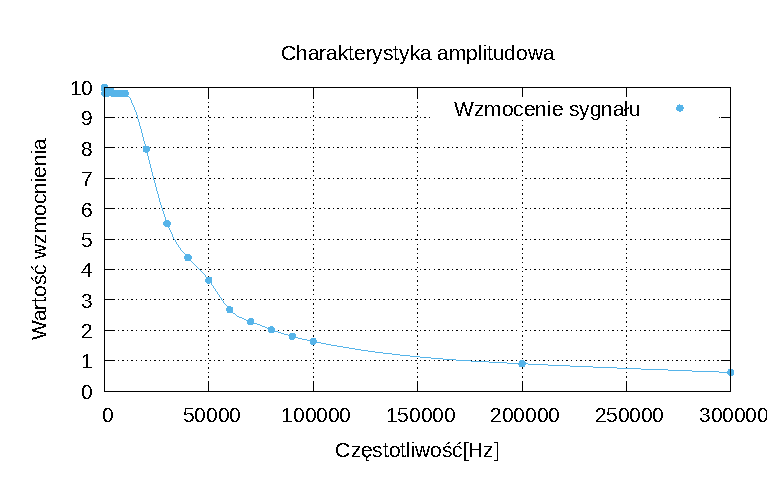
\includegraphics[scale=1]{grafiki/amp_plot.eps}
        \caption{Charakterystyka amplitudowa generatora odwracającego fazę o wzmocnieniu 10,
        \\Źródło: Opracowanie własne}
      \end{figure}

      Jak widzimy wraz ze wzrostem częstotliwości z czasem wzmocnienie układu opada. Jest to spodziewane zjawisko co oznacza, że układ zachowuje się poprawnie.

      \subsubsection{Charakterystyka fazowa}

      \begin{table}[!ht]
        \begin{minipage}{.5\textwidth}
          \centering
          \scalebox{0.65}{
          \begin{tabular}{|c|c|}
          \hline
          \textbf{Hz} & \textbf{Faza[stopnie]} \\
          \hline
          100 & 179.4 \\
          200 & 177.9 \\
          300 & 179.6 \\
          400 & 178.8 \\
          500 & 178 \\
          600 & 176.8 \\
          700 & 177.1 \\
          800 & 179.6 \\
          900 & 179 \\
          1000 & 177.9 \\
          2000 & 178.5 \\
          3000 & 175.9 \\
          4000 & 176.6 \\
          5000 & 175.6 \\
          6000 & 173 \\
          7000 & 173.5 \\
          8000 & 172.8 \\
          9000 & 167.5 \\
          10000 & 167.5 \\
          20000 & 136.2 \\
          30000 & 118.7 \\
          40000 & 114.5 \\
          50000 & 109.4 \\
          60000 & 98.2 \\
          70000 & 103.5 \\
          80000 & 91.03 \\
          90000 & 100.1 \\
          100000 & 93.51 \\
          200000 & 88.56 \\ 
          300000 & -106.3 \\
          \hline
          \end{tabular}}
          \caption{Dane odczytane z oscyloskopu,
          \\Źródło: Opracowanie własne}
          \label{Tabela2}
        \end{minipage}%
        \begin{minipage}{.5\textwidth}
          \centering
          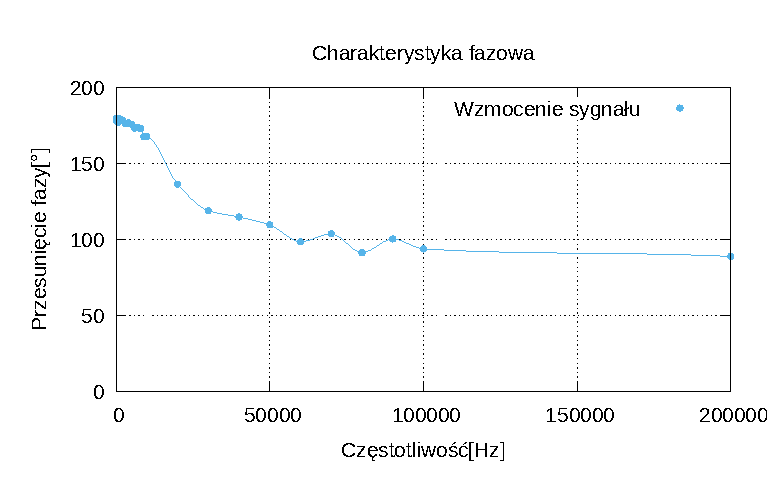
\includegraphics[scale=0.75]{grafiki/phase_plot.eps}
          \captionof{figure}{Charakterystyka fazowa generatora odwracającego fazę o wzmocnieniu 10,
              \\Źródło: Opracowanie własne}
        \end{minipage}
      \end{table}

      Jak jesteśmy wstanie zaobserwować, podobna charakterystyka tyczy się fazy układu. Dla niższych częstotliwości utrzymuje się ona w okolicach oczekiwanych $180^\circ$ jednak wraz ze wzrostem częstotliwości obserwujemy zmniejszanie się przesunięcia.

    \subsection{Ćwiczenie 3.3}
      Następnym układem do zmontowania był sumator o dwóch wejściach. Jego budowa składała się z 3 oporników. Trzymając się oznaczeń ze schematu(\ref{fig2:sumujacy}), zanotowałem poniższe wartości dla wybranych oporników:\\
      $R = 99,6k\Omega$ \\
      $R_1 = 9,97k\Omega$ \\
      $R_2 = 9,97k\Omega$ \\

      \begin{figure}[!ht]
        \centering
        \includegraphics[scale=0.07]{grafiki/plytka_sumujący.jpg}
        \caption{Poprawnie zmontowany sumator o dwóch wejściach,
        \\Źródło: Opracowanie własne}
      \end{figure}

      \subsubsection{Zjawisko dudnień}
        Zaobserwowanie powyższego zjawisko można osiągnąć sumując dwa sygnały o podobnych amplitudach oraz nieznacznie różnych częstotliwościach. Oto przy jakich ustawiniach udało się to zjawisko zaobserwować:

        \begin{table}[h]
          \centering
          \scalebox{0.65}{
          \begin{tabular}{|c|c|c|c|}
          \hline
          \textbf{Kanał z generatora} & \textbf{Odpowiadający opornik} & \textbf{Częstotliwość} & \textbf{Amplituda} \\
          \hline
          ch1 & $R_1$ & 11kHz & 0,5V \\
          ch2 & $R_2$ & 10kHz & 0,5V \\
          \hline
          \end{tabular}}
          \caption{Ustawienia dla których wystapiło zjawisko dudnień, \\Źródło: Opracowanie własne}
          \label{Tabela3}
      \end{table}

      \begin{figure}[!ht]
        \centering
        \includegraphics[scale=0.65]{grafiki/freq.png}
        \caption{Zjawisko dudnień uzyskane przy zastosowaniu nieznacznie różnych częstotliwości,
        \\Źródło: Opracowanie własne}
      \end{figure}

      Pomiary uzyskane podczas zajęć prezentują się nastepująco: \\
      Obwiednia: $\mathbf{990,1Hz}$ \\
      Sygnał zsumowany: $\mathbf{\sim10V}$ \\

      Wynik uzyskany dla obwiedni jest poprawny dla danych wejściowych:
      \begin{equation}
        11kHz - 10kHz = 1kHz
      \end{equation}

      Natomiast obserwując maksymalną amplitudę dudnień jesteśmy wstanie zauważyć, że wynosi ona $\sim 10V$. Zestawiając to ze wzorem(\ref{eq2:sumujacy}):
      \begin{equation}
        U_{WY} = -99.6k\Omega(\frac{0,5V}{9.97k\Omega}+\frac{0,5V}{9.97k\Omega}) = - 9,98996...V \approx - 10V
      \end{equation}
      Zgadza się to jak najbardziej z wartościami które osiąga uzykane w eksperymencie zjawisko dudnienia.

      
    \subsection{Ćwiczenie 3.4}
      Kolejna modyfikacja układu dotyczyła jego przebudowy w przerzutnik Schmidta. Do jego budowy zostały zastosowane wbudowane w płytkę oporniki o zmiennej oporności. ich maksymalne oporności wynosiły $100\Omega$ oraz $10\Omega$. Dokładną wartość obu można dostosować obracając specjalne pokrętła.

      \begin{figure}[!ht]
        \centering
        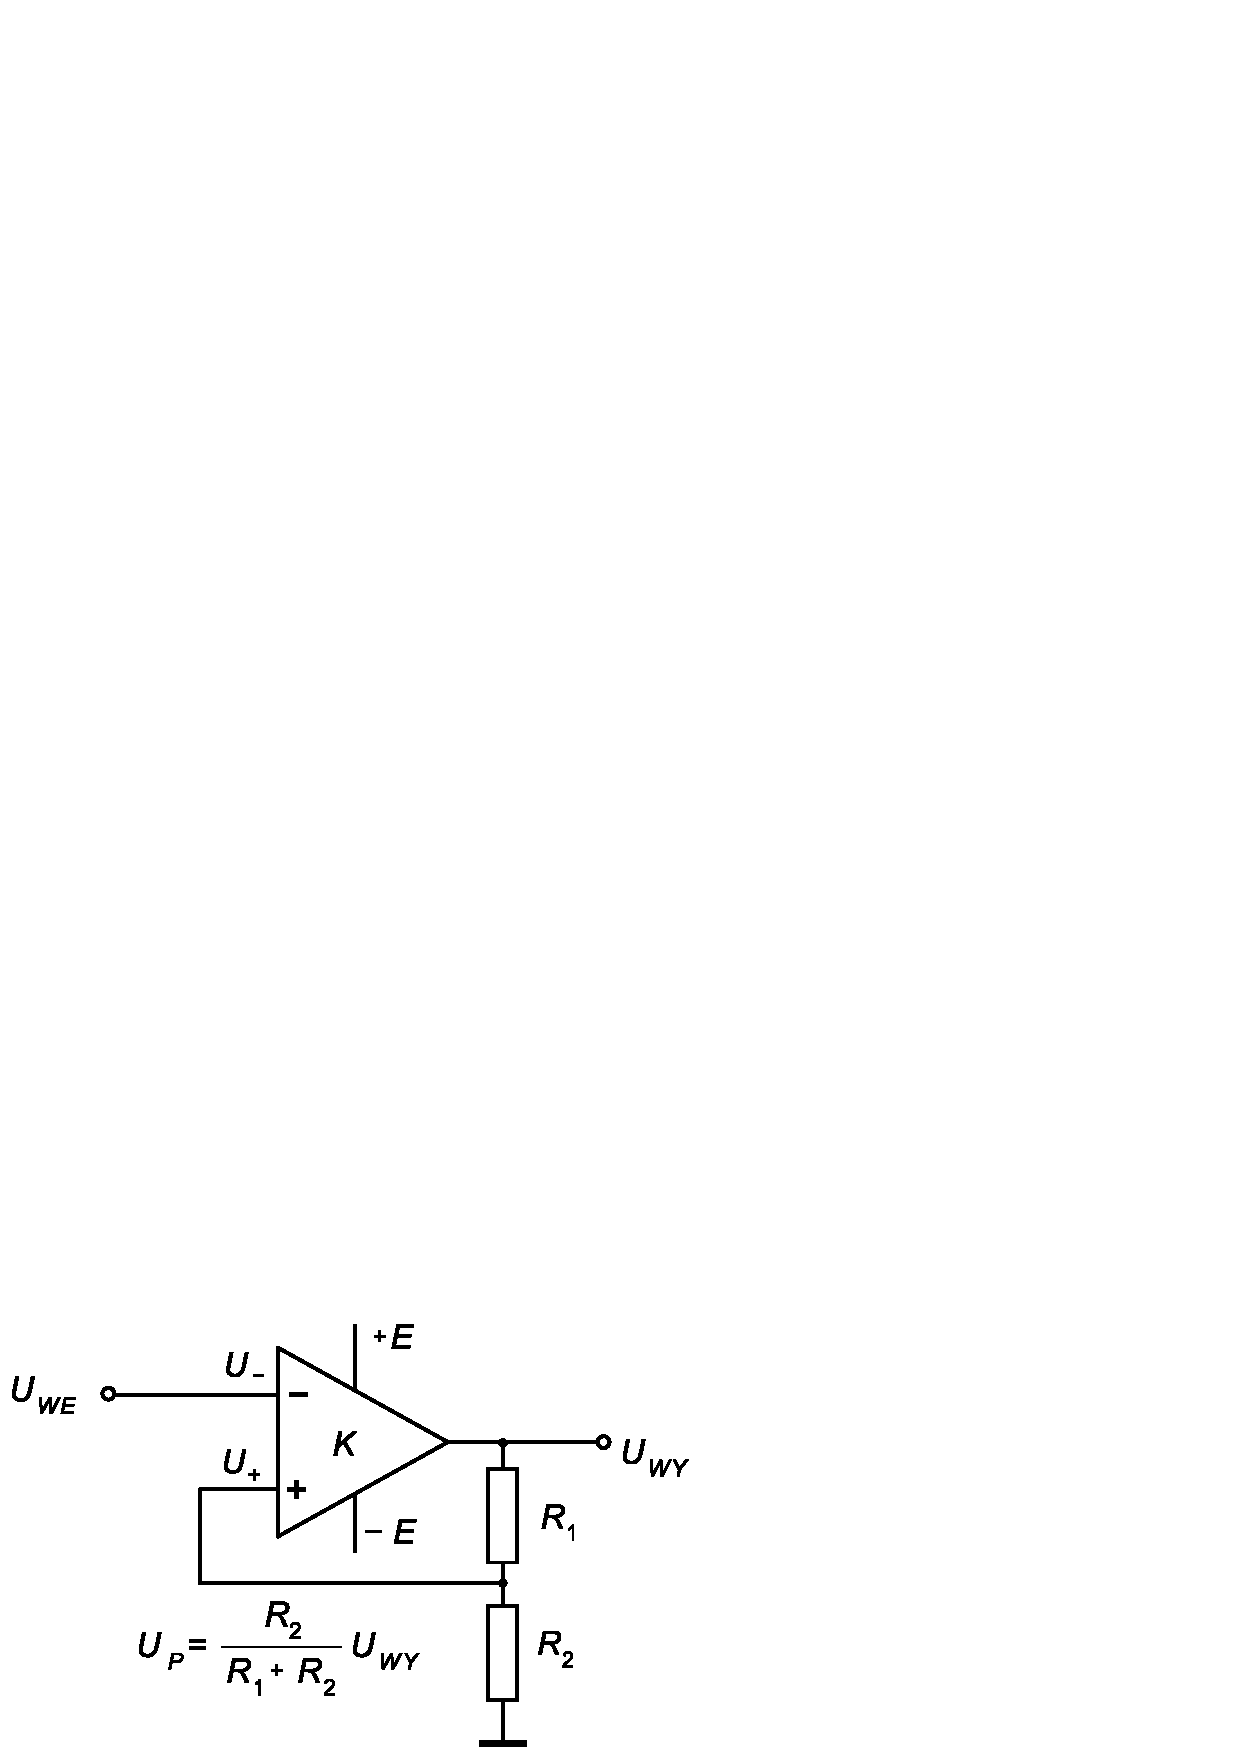
\includegraphics[scale=0.07]{grafiki/Schmidt.jpg}
        \caption{Poprawnie zmontowany przerzutnik Schmidta korzystający z oporników ze zmienną opornością,
        \\Źródło: Opracowanie własne}
      \end{figure}

    Dynamiczna możliwość zmiany oporu została wykorzystana do poprawnego pozycjonowania sygnałów na podziałce na oscyloskopie w celu łatwiejszych pomiarów. Korzystając z oznaczeń na schemacie(\ref{fig6:Schmidt}) ustawione wartości oporników prezetują się nastepująco: \\
    $R_1 = 0,971k\Omega$ \\
    $R_2 = 97,1k\Omega$ \\

    Kolejnym krokiem było uzyskanie efektu histerezy wykreślając sygnał wejściowych i wyjściowy na osiach X oraz Y. Powyższe kroki należało wykonać dla fal sinusoidalnych oraz trójkątnych.

    Korzystając z ozanczeń(\ref{fig7:histereza}) oraz wzoru na schemacie(\ref{fig6:Schmidt}) możemy podjąć się obliczeń:\\
    \begin{equation}
      U_P = \frac{97,1\Omega}{0,971k\Omega+9,71\Omega} \cdot 11,88V = 1,08V
    \end{equation}

    \subsubsection{Sygnał sinusoidalny}

      \begin{figure}[!ht]
        \begin{minipage}{.5\textwidth}
            \centering
            \includegraphics[scale=0.35]{grafiki/sin_wyj.png}
            \caption{Zestawienie sygnału wejściowego z wyjściowym dla fali sinusoidalnej,
            \\Źródło: Opracowanie własne}
        \end{minipage}
        \begin{minipage}{.5\textwidth}
            \centering
            \includegraphics[scale=0.35]{grafiki/sin_Histereza.png} 
            \caption{Uzyskane zjawisko histerezy w widoku XY oscyloskopu dla fali sinusoidalnej,
            \\Źródło: Opracowanie własne}
        \end{minipage}
      \end{figure}
      \pagebreak

    \subsubsection{Sygnał trójkątny}

      \begin{figure}[!ht]
        \begin{minipage}{.5\textwidth}
            \centering
            \includegraphics[scale=0.35]{grafiki/ramp_wyj.png}
            \caption{Zestawienie sygnału wejściowego z wyjściowym dla fali trójkątnej,
            \\Źródło: Opracowanie własne}
        \end{minipage}
        \begin{minipage}{.5\textwidth}
            \centering
            \includegraphics[scale=0.35]{grafiki/ramp_Histereza.png} 
            \caption{Uzyskane zjawisko histerezy w widoku XY oscyloskopu dla fali trójkątnej,
            \\Źródło: Opracowanie własne}
        \end{minipage}
      \end{figure}

  \section{Omówienie wyników}
    \subsection{Ćwiczenie 3.1}
      Wszystkie pomiary zgadzały się z oczekiwanymi.
    \subsection{Ćwiczenie 3.2}
      Wartości oporników oraz obliczone wzmocnienie co do wartości zgadzały z uzyskanym efektem co sugeruje poprawność działania układu. Jednak szczegółem dosyć martwiącym jest odczyt uzyskanej amplitudy(wejściowej jak i wyjściowej). Posiadają one bowiem wartość podwojoną do wprowadzonej(1V). Domyślam się, że jest to mój błąd spowodowany brakiem włączenia specyficznego ustawienia którego nazewnictwa nie jestem wstanie przytoczyć(sprawiało ono, że przekazywana była faktyczna wartość a nie podwojona). Występowało ono kilka razy na poprzednich zajęciach jednakże tym razem musiałem to przeoczyć podczas wykonywania eksperymentów.
      Nie zmienia to jednak faktu poprawności wykonanego układu oraz pozostałych odczytów jak przesunięcie fazy które oscylowało w okolicy $180^\circ$. Wyniki uzyskane przy zbieraniu charakterystyk układu dotyczyły wartości wzmocnienia oraz przesunięcia fazowego w zależności od częstotliwości więc na te dane nie wpłynęło to w żaden negatywny sposób.

    \subsection{Ćwiczenie 3.3}
      Zadanie to przeszło pomyślnie od poczatku do końca. Udało się zaobserwować pożądany efekt dudnień oraz wszystkie wykonane obliczenia pokrywają się z danymi z oscyloskopu.

    \subsection{Ćwiczenie 3.4}
      Jak można zauważyć po przebiegu sygnałów dla obu typów fal, przerzutnik działa poprawnie -- zmienia swój stan gdy osiagniemy odpowiednią amplitudę. Jednak spoglądając na wyniki obliczeń oraz pomiary histerezy znowu jesteśmy wstanie zauważyć pewną różnicę wyników. Jest to zapewne spowodowane tym samym powodem o którym wspomniałem wcześniej. Proste podzielenie przez 2 daje nam już zbliżone wartości do wykonanych obliczeń oraz pomiarów $U_P$ oraz $E$.
      
  \section{Podsumowanie}
    Podczas powyżej opisanych zajęć laboratoryjnych zgłębione zostało działanie wzmacniaczy operacyjnych oraz przerzutników, które stanowią fundamentalne elementy w dziedzinie elektroniki. W praktyce zbudowane były różne typy układów wzmacniaczy, takie jak\textit{wzmacniacz odwracający fazę}, który charakteryzuje się przesunięciem fazowym na wyjściu o 180 stopni w stosunku do sygnału wejściowego, czy \textit{sumator dwóch sygnałów}.
    Ponadto w kontekście przerzutników przeprowadzona została analiza \textit{przerzutnika Schmidta}. Zbudowany układ umożliwił zrozumienie istoty histerezy oraz zjawiska przełączania stanu na podstawie poziomu napięcia wejściowego. To doświadczenie pozwoliło lepiej zrozumieć praktyczne zastosowania przerzutników w układach, gdzie zachowanie takie ma kluczowe znaczenie dla stabilnego działania systemu.

  \section{Notatki i materiały z zajęć}

    \begin{figure}[!ht]
      \begin{minipage}{.5\textwidth}
          \centering
          \includegraphics[scale=0.2]{grafiki/zdj1.jpg}
          \caption{Wypełniona karta pracy,
          \\Źródło: Opracowanie własne}
      \end{minipage}
      \begin{minipage}{.5\textwidth}
          \centering
          \includegraphics[scale=0.2]{grafiki/zdj2.jpg} 
          \caption{Wypełniona karta pracy,
          \\Źródło: Opracowanie własne}
      \end{minipage}
    \end{figure}

    \begin{figure}[!ht]
      \begin{minipage}{.5\textwidth}
          \centering
          \includegraphics[scale=0.15]{grafiki/zdj3.jpg}
          \caption{Wypełniona karta pracy,
          \\Źródło: Opracowanie własne}
      \end{minipage}
      \begin{minipage}{.5\textwidth}
          \centering
          \includegraphics[scale=0.08]{grafiki/r_min.jpg} 
          \caption{Minimalny opór opornika $R_1$ z płytki,
          \\Źródło: Opracowanie własne}
      \end{minipage}
    \end{figure}

    \begin{figure}[!ht]
      \begin{minipage}{.5\textwidth}
          \centering
          \includegraphics[scale=0.08]{grafiki/r_max.jpg}
          \caption{Maksymalny opór opornika $R_1$ z płytki,
          \\Źródło: Opracowanie własne}
      \end{minipage}
      \begin{minipage}{.5\textwidth}
          \centering
          \includegraphics[scale=0.08]{grafiki/y_min.jpg} 
          \caption{Minimalny opór opornika $R_2$ z płytki,
          \\Źródło: Opracowanie własne}
      \end{minipage}
    \end{figure}

    \begin{figure}[!ht]
      \centering
      \includegraphics[scale=0.125]{grafiki/y_max.jpg}
      \caption{Maksymalny opór opornika $R_1$ z płytki,
      \\Źródło: Opracowanie własne}
    \end{figure}


\end{document}